\documentclass[11pt,a4paper]{article}

\usepackage{fontspec}
\setmainfont{DejaVu Serif}[ItalicFont={DejaVu Serif}, ItalicFeatures={FakeSlant=0.2}, BoldItalicFont={DejaVu Serif Bold}, BoldItalicFeatures={FakeSlant=0.2}]
\setsansfont{DejaVu Sans}
\setmonofont{DejaVu Sans Mono}[Scale=0.85]
\usepackage[margin=2.1cm,headheight=14pt]{geometry}
\usepackage{graphicx}
\usepackage[table]{xcolor}
\usepackage{listings}
\usepackage[most]{tcolorbox}
\usepackage{booktabs}
\usepackage{tabularx}
\usepackage{enumitem}
\usepackage{titlesec}
\usepackage{fancyhdr}
\usepackage[hidelinks]{hyperref}
\usepackage{float}
\usepackage{caption}
\usepackage{amssymb}
\usepackage{tikz}
\usetikzlibrary{positioning,arrows.meta,fit,backgrounds}
\usepackage{multicol}
\usepackage{tocloft}
\usepackage{needspace}
\usepackage{etoolbox}

\setlength{\cftbeforesecskip}{3pt}
\setlength{\cftbeforesubsecskip}{0pt}

\setlength{\cftsubsecindent}{2.2em}
\setlength{\cftsubsecnumwidth}{2.8em}
\setlength{\cftsecnumwidth}{2.2em}
\renewcommand{\cftsubsecfont}{\small}
\renewcommand{\cftsubsecpagefont}{\small}
\renewcommand{\cfttoctitlefont}{\LARGE\sffamily\bfseries\color{accent}}

\definecolor{accent}{HTML}{1F6FEB}
\definecolor{cmdbg}{HTML}{0D1117}
\definecolor{cmdfg}{HTML}{E6EDF3}
\definecolor{outbg}{HTML}{F6F8FA}
\definecolor{outframe}{HTML}{D0D7DE}
\definecolor{notebg}{HTML}{EAF2FE}
\definecolor{rowbg}{HTML}{F1F4F8}
\setlength{\aboverulesep}{0pt}
\setlength{\belowrulesep}{0pt}
\setlength{\heavyrulewidth}{1pt}
\renewcommand{\arraystretch}{1.2}
\AtBeginEnvironment{tabularx}{\rowcolors{2}{white}{rowbg}}
\newcommand{\doc}[2]{\href{https://rechefe.github.io/ipu-emulator/dev/#1/}{\textcolor{accent}{#2}}}
\definecolor{muted}{HTML}{57606A}

\titleformat{\section}{\LARGE\sffamily\bfseries\color{accent}}{\thesection}{0.7em}{}
\titleformat{\subsection}{\large\sffamily\bfseries}{\thesubsection}{0.7em}{}
\titlespacing*{\section}{0pt}{0pt}{0.8em}
\newcommand{\sectionbreak}{\clearpage}
\setlength{\parindent}{0pt}
\setlength{\parskip}{0.55em}
\captionsetup{font={small,sf},labelfont=bf,skip=4pt}
\setlength{\textfloatsep}{8pt}

\pagestyle{fancy}
\fancyhf{}
\fancyhead[L]{\sffamily\small\color{muted}IPU Emulator --- Getting Started}
\fancyhead[R]{\sffamily\small\color{muted}\nouppercase{\leftmark}}
\fancyfoot[C]{\sffamily\small\thepage}
\renewcommand{\headrulewidth}{0.3pt}

\lstdefinestyle{shell}{
  aboveskip=0pt, belowskip=0pt,
  basicstyle=\ttfamily\small\bfseries\color{white},
  breaklines=true, columns=fullflexible, keepspaces=true,
  showstringspaces=false, upquote=true,
  postbreak=\mbox{\textcolor{muted}{$\hookrightarrow$}\space},
}
\lstdefinestyle{output}{
  aboveskip=0pt, belowskip=0pt,
  basicstyle=\ttfamily\scriptsize\color{termfg},
  breaklines=true, columns=fullflexible, keepspaces=true,
  showstringspaces=false, upquote=true,
  postbreak=\space\space\space\space,
}
\lstdefinestyle{tree}{
  aboveskip=0pt, belowskip=0pt,
  basicstyle=\ttfamily\footnotesize\color{black},
  breaklines=true, columns=fullflexible, keepspaces=true,
  showstringspaces=false, upquote=true,
}
\lstdefinestyle{code}{
  basicstyle=\ttfamily\footnotesize,
  breaklines=true, columns=fullflexible, keepspaces=true,
  showstringspaces=false, language=Python, upquote=true,
  keywordstyle=\color{accent}\bfseries, commentstyle=\color{muted}\itshape,
  stringstyle=\color{teal},
}

\definecolor{termbg}{HTML}{1E1E1E}
\definecolor{termbar}{HTML}{323233}
\definecolor{termband}{HTML}{005F87}
\definecolor{termfg}{HTML}{D4D4D4}
\definecolor{dotr}{HTML}{FF5F57}
\definecolor{doty}{HTML}{FEBC2E}
\definecolor{dotg}{HTML}{28C840}
\newcommand{\termdots}{\tikz[baseline=-0.6ex]{\fill[dotr] (0,0) circle (0.8mm);
  \fill[doty] (2.8mm,0) circle (0.8mm); \fill[dotg] (5.6mm,0) circle (0.8mm);}}
\tcbset{termwin/.style={enhanced, colframe=termbar, boxrule=0pt, arc=4pt,
  left=8pt, right=8pt, top=3pt, bottom=3pt,
  colbacktitle=termbar, coltitle=termfg!70, fonttitle=\sffamily\scriptsize,
  toptitle=0.4mm, bottomtitle=0.4mm,
  title={\termdots\hfill terminal\hfill\phantom{\termdots}}}}
\newtcblisting{termcmd}{listing only, listing options={style=shell},
  termwin, colback=termband}
\newtcblisting{termcmdtop}{listing only, listing options={style=shell},
  termwin, colback=termband, sharp corners=south, after skip=0pt}
\newtcblisting{termout}{listing only, listing options={style=output},
  enhanced, colback=termbg, colframe=termbg, boxrule=0pt, arc=4pt,
  sharp corners=north, before skip=0pt, left=8pt, right=8pt, top=4pt, bottom=5pt,
  before={\par\vspace*{-\parskip}}}
\newtcblisting{filetree}{listing only, listing options={style=tree},
  enhanced, colback=outbg, colframe=muted, boxrule=0.6pt, arc=4pt,
  left=8pt, right=8pt, top=4pt, bottom=4pt,
  attach boxed title to top left={xshift=8pt,yshift=-2pt},
  boxed title style={colback=outframe, colframe=outframe, arc=2pt},
  coltitle=black, fonttitle=\sffamily\scriptsize\bfseries, title={files}}
\newtcblisting{pycode}{listing only, listing options={style=code},
  enhanced, colback=outbg, colframe=outframe, boxrule=0.5pt, arc=4pt,
  left=8pt, right=8pt, top=4pt, bottom=4pt}
\newtcolorbox{note}{enhanced, breakable, colback=notebg, colframe=accent,
  boxrule=0pt, leftrule=3pt, arc=0pt, left=8pt, right=8pt, top=4pt, bottom=4pt}

\newcommand{\terminal}[3][0.75]{%
  \begin{figure}[H]\centering
  \includegraphics[width=#1\linewidth]{images/#2}
  \caption{#3}
  \end{figure}}
\newcommand{\screenshot}[3][0.72]{%
  \begin{figure}[H]\centering
  \includegraphics[width=#1\linewidth]{images/#2}
  \caption{#3}
  \end{figure}}

\begin{document}
\sloppy
\begin{titlepage}
\centering
\vspace*{2.5cm}
{\sffamily\bfseries\Huge\color{accent} IPU Emulator\par}
\vspace{0.4cm}
{\sffamily\LARGE Getting Started\par}
\vspace{0.3cm}
{\sffamily\large\color{muted} Finding, running, testing and debugging kernels\par}
\vspace{0.3cm}
{\sffamily\small\color{muted} Written by Yarden Carmi\par}
{\sffamily\small\color{muted} Last updated \today\par}
\vspace{1.5cm}
% images/cover.svg is the editable source (a Lucid export); regenerate the PDF with
% `mutool convert -o images/cover.pdf images/cover.svg` after editing it.
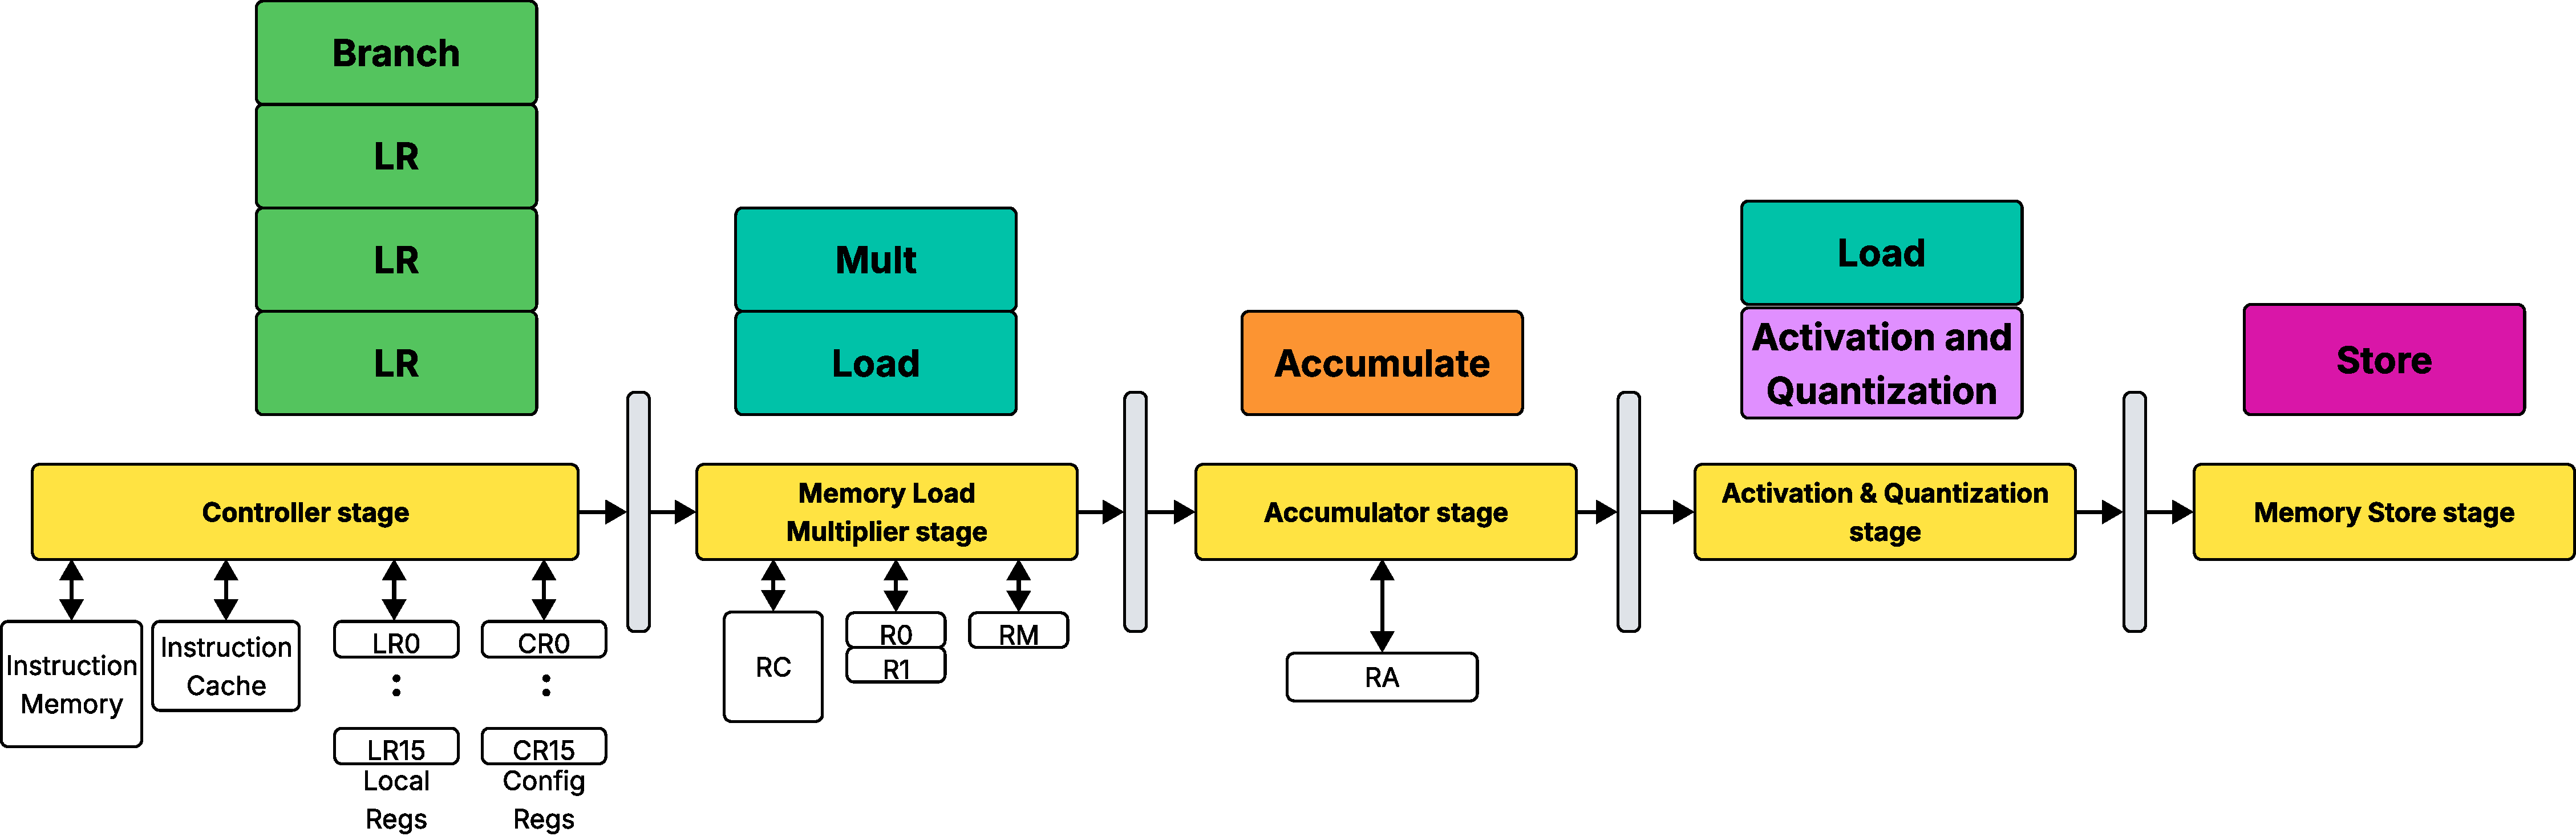
\includegraphics[width=\linewidth]{images/cover.pdf}
\vfill
{\sffamily\small\color{muted} Repository: \href{https://github.com/rechefe/ipu-emulator}{\textcolor{accent}{github.com/rechefe/ipu-emulator}}\par}
{\sffamily\small\color{muted} Documentation: \href{https://rechefe.github.io/ipu-emulator/}{\textcolor{accent}{rechefe.github.io/ipu-emulator}}\par}
\end{titlepage}
\tableofcontents
\newpage

%======================================================================
\section{What the IPU emulator is for}

The IPU is a vector processor for neural-network inference. It runs
\textbf{kernels}.

\subsection{What a kernel is}

A kernel computes one operation --- a convolution, a matrix
multiply, a softmax, a layer norm --- for a range of shapes, and consists of:

\begin{itemize}
\item an IPU assembly program (\texttt{.asm});
\item a description, \texttt{kernel.toml}, from which the harness places the
  inputs in the IPU's memory, sets the control registers, and reads the
  result back after the run;
\item cases: named inputs, each with a NumPy reference the result must match.
\end{itemize}

\subsection{Example: MobileViT-S}\label{sec:mvit}

A network runs as a chain of kernels, each reading the previous one's output
from memory. MobileViT-S is one such network. Its convolutional part is built
from MV2 blocks ($1\times1$ expand,
$3\times3$ depthwise, $1\times1$ project, residual add), which run on the
convolution kernels and \texttt{residual\_add}. Its transformer part:

\begin{figure}[H]\centering
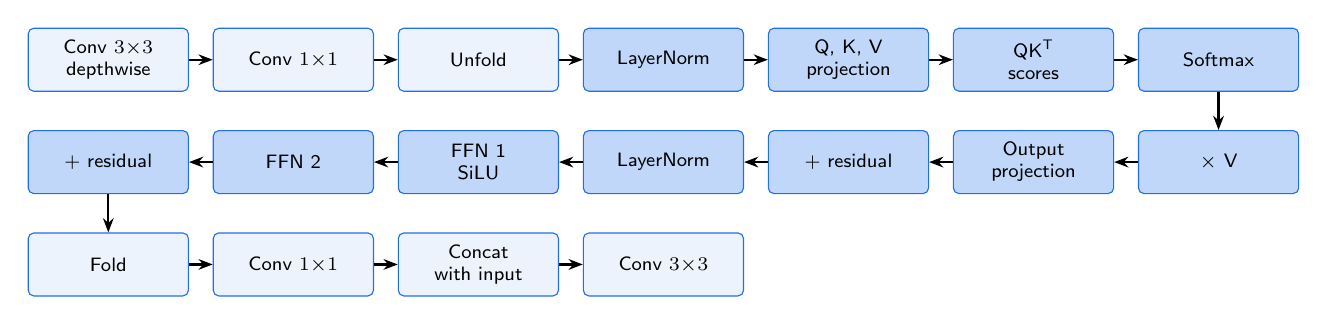
\begin{tikzpicture}[
  k/.style={draw=accent, fill=accent!8, rounded corners=2pt, minimum height=8mm,
            minimum width=19mm, text width=18mm, align=center, font=\sffamily\scriptsize},
  t/.style={k, fill=accent!28},
  arr/.style={-{Stealth[length=1.8mm]}, thick}]
\foreach \n/\s/\l [count=\i from 0] in
  {a0/k/{Conv $3{\times}3$\\depthwise}, a1/k/{Conv $1{\times}1$}, a2/k/Unfold,
   a3/t/LayerNorm, a4/t/{Q, K, V\\projection}, a5/t/{QK$^\mathsf{T}$\\scores}, a6/t/Softmax}
  \node[\s] (\n) at (\i*23.5mm, 0) {\l};
\foreach \n/\s/\l [count=\i from 0] in
  {b6/t/{$\times$ V}, b5/t/{Output\\projection}, b4/t/{+ residual}, b3/t/LayerNorm,
   b2/t/{FFN 1\\SiLU}, b1/t/{FFN 2}, b0/t/{+ residual}}
  \node[\s] (\n) at ({(6-\i)*23.5mm}, -13mm) {\l};
\foreach \n/\l [count=\i from 0] in
  {c0/Fold, c1/{Conv $1{\times}1$}, c2/{Concat\\with input}, c3/{Conv $3{\times}3$}}
  \node[k] (\n) at (\i*23.5mm, -26mm) {\l};
\foreach \x/\y in {a0/a1,a1/a2,a2/a3,a3/a4,a4/a5,a5/a6,a6/b6,b6/b5,b5/b4,b4/b3,b3/b2,b2/b1,b1/b0,b0/c0,c0/c1,c1/c2,c2/c3}
  \draw[arr] (\x) -- (\y);
\end{tikzpicture}
\caption{\label{fig:mvit}A MobileViT-S transformer layer. Dark boxes: the transformer block, run twice.}
\end{figure}

Each box is one kernel run; where a box lists two kernels, either implements
that step (\doc{kernels/mobilevit}{MobileViT-S kernels} lists every layer):

\begin{center}
\footnotesize\renewcommand{\arraystretch}{1.0}
\begin{tabularx}{\linewidth}{lX}
\toprule
Box & Kernels (layer 3: $d=144$, 256 tokens) \\
\midrule
Conv $3\times3$ depthwise & \texttt{depthwise\_conv\_universal} \\
Conv $1\times1$ & \texttt{pointwise\_conv\_unified} \\
Unfold & \texttt{unfold\_32x32x144} \\
LayerNorm & \texttt{layernorm\_256x144} \\
Q, K, V projection & \texttt{proj\_qkv\_144\_p4}, \texttt{matmul\_432x144\_x128} \\
QK$^\mathsf{T}$ scores & \texttt{qk\_scores\_256x36}, \texttt{attn\_scores\_km\_256x36} \\
Softmax & \texttt{softmax\_rows\_long} (query-major), \texttt{softmax\_columns} (key-major) \\
$\times$ V & \texttt{attn\_v\_256x36}, \texttt{attn\_v\_bcast\_36} \\
Output projection & \texttt{proj\_outproj\_144\_p4}, \texttt{matmul\_144x144\_x128} \\
+ residual & \texttt{residual\_add\_256x144} \\
FFN 1, FFN 2 & \texttt{proj\_ffn1\_144\_p4}, \texttt{proj\_ffn2\_144\_p4} \\
Fold & \texttt{fold\_32x32x144} \\
Concat & \texttt{concat\_32x32x96x96} \\
Conv $3\times3$ & \texttt{conv\_universal} \\
\bottomrule
\end{tabularx}
\end{center}

%======================================================================
\section{The IPU architecture}

Hardware specifications: \doc{specs/ARCH-stage-ctrl}{control stage},
\doc{specs/ARCH-stage-mult}{multiply stage}, \doc{specs/ARCH-stage-acc}{accumulator stage}, \doc{specs/ARCH-stage-aaq-str}{AaQ stage},
\doc{specs/cache-unit}{cache unit}, \doc{specs/riscv-host-integration}{RISC-V host integration}.

\subsection{System}

\begin{figure}[H]\centering
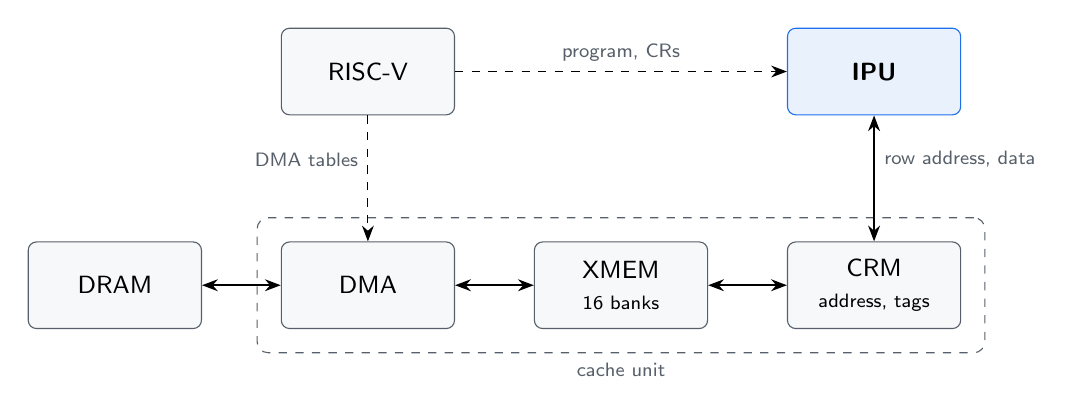
\begin{tikzpicture}[
  blk/.style={draw=accent, fill=accent!10, rounded corners=3pt, minimum height=11mm,
              minimum width=22mm, align=center, font=\sffamily\small},
  ext/.style={draw=muted, fill=outbg, rounded corners=3pt, minimum height=11mm,
              minimum width=22mm, align=center, font=\sffamily\small},
  dp/.style={{Stealth[length=2mm]}-{Stealth[length=2mm]}, thick},
  ctl/.style={-{Stealth[length=2mm]}, dashed},
  lab/.style={font=\sffamily\scriptsize, text=muted}]
\node[ext] (dram) {DRAM};
\node[ext, right=10mm of dram] (dma) {DMA};
\node[ext, right=10mm of dma] (xmem) {XMEM\\\scriptsize 16 banks};
\node[ext, right=10mm of xmem] (crm) {CRM\\\scriptsize address, tags};
\node[blk, above=16mm of crm] (ipu) {\textbf{IPU}};
\node[ext, above=16mm of dma] (riscv) {RISC-V};
\draw[dp] (dram) -- (dma);
\draw[dp] (dma) -- (xmem);
\draw[dp] (xmem) -- (crm);
\draw[dp] (ipu) -- node[lab, right, pos=0.35]{row address, data} (crm);
\draw[ctl] (riscv) -- node[lab, above]{program, CRs} (ipu);
\draw[ctl] (riscv) -- node[lab, left, pos=0.35]{DMA tables} (dma);
\begin{scope}[on background layer]
\node[draw=muted, dashed, rounded corners=4pt, inner sep=3mm, fit=(dma)(xmem)(crm),
      label={[lab]below:cache unit}] {};
\end{scope}
\end{tikzpicture}
\caption{The IPU in its system (solid: data, dashed: control).}
\end{figure}

\subsection{The pipeline}

\begin{figure}[H]\centering
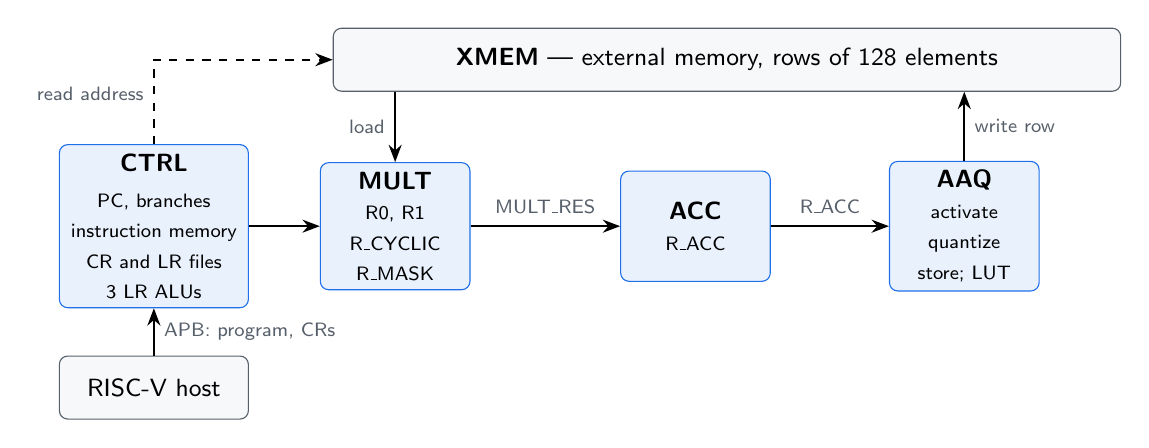
\begin{tikzpicture}[
  stage/.style={draw=accent, fill=accent!10, rounded corners=3pt, minimum height=14mm,
                minimum width=19mm, align=center, font=\sffamily\small},
  mem/.style={draw=muted, fill=outbg, rounded corners=3pt, minimum height=8mm,
              align=center, font=\sffamily\small},
  arr/.style={-{Stealth[length=2.2mm]}, thick},
  lab/.style={font=\sffamily\scriptsize, text=muted}]
\node[stage, minimum width=24mm, minimum height=20mm] (ctrl)
  {\textbf{CTRL}\\[2pt]\scriptsize PC, branches\\\scriptsize instruction memory\\\scriptsize CR and LR files\\\scriptsize 3 LR ALUs};
\node[stage, right=9mm of ctrl] (mult) {\textbf{MULT}\\\scriptsize R0, R1\\\scriptsize R\_CYCLIC\\\scriptsize R\_MASK};
\node[stage, right=19mm of mult] (acc) {\textbf{ACC}\\\scriptsize R\_ACC};
\node[stage, right=15mm of acc] (aaq) {\textbf{AAQ}\\\scriptsize activate\\\scriptsize quantize\\\scriptsize store; LUT};
\node[mem, above=10mm of acc, minimum width=100mm, xshift=4mm] (xmem) {\textbf{XMEM} --- external memory, rows of 128 elements};
\node[mem, below=6mm of ctrl, minimum width=24mm] (host) {RISC-V host};
\draw[arr] (host) -- node[lab, right]{APB: program, CRs} (ctrl);
\draw[arr] (ctrl) -- (mult);
\draw[arr] (mult) -- node[lab, above=1pt]{MULT\_RES} (acc);
\draw[arr] (acc) -- node[lab, above=1pt]{R\_ACC} (aaq);
\draw[arr, dashed] (ctrl.north) |- node[lab, pos=0.3, left]{read address} (xmem.west);
\draw[arr] (xmem.south -| mult.north) -- node[lab, left]{load} (mult.north);
\draw[arr] (aaq.north) -- node[lab, right]{write row} (xmem.south -| aaq.north);
\end{tikzpicture}
\caption{The pipeline. CTRL issues one instruction word per cycle; the AAQ
stage writes its result to XMEM itself.}
\end{figure}

\subsection{Memory and run modes}

\textbf{XMEM} is the external memory. Assembly addresses it in \emph{rows} of
128 elements, and every load and store moves exactly one row. A run is in one
of two \textbf{modes}, chosen when it starts; the program and its row numbers
are the same in both (\doc{explanation/element-formats}{Element formats}):

\begin{center}
\begin{tabularx}{\linewidth}{lX}
\toprule
Mode & A row holds \\
\midrule
\textbf{NX8} (hardware) & 128 NX8 elements (128 bytes) and a 16-bit metadata
word: the row's \texttt{scale} and \texttt{dynamic\_exponent}. An element's
value depends on the row's scale and on a \emph{QF} (quantization format) that
the instruction names. \\
\textbf{FP32} (emulator only) & 128 IEEE float32 elements (512 bytes), with no
metadata, no scaling and no quantization. It runs a kernel written for NX8 at
full precision, for debugging and for comparing with a reference. \\
\bottomrule
\end{tabularx}
\end{center}

FP32 and NX8 are the only element formats; a kernel names an NX8 variant by
its type, such as \texttt{e4}, \texttt{e5} or \texttt{dynamic}. In both modes
\texttt{MULT\_RES} and \texttt{R\_ACC} hold FP32: in NX8 the multiplier expands
each element to FP32 first, and the AAQ stage quantizes the result back when
it stores it.

\needspace{7cm}
\subsection{Registers}

\begin{center}
\begin{tabularx}{\linewidth}{l>{\raggedright\arraybackslash}p{0.3\linewidth}X}
\toprule
Register & Holds & Role \\
\midrule
\texttt{R0}, \texttt{R1} & one row each, and its metadata & multiply-stage operands \\
\texttt{R\_CYCLIC} & 512 elements & ring of four 128-element slots, each with its row's metadata \\
\texttt{R\_MASK} & 8 masks of 128 bits & one enable bit per lane \\
\texttt{MULT\_RES} & 128 $\times$ FP32 & result of the multiply stage \\
\texttt{R\_ACC} & 128 $\times$ FP32 & accumulator \\
AaQ LUT & 5 segments of 1024 bits & the table the hardware evaluates \texttt{generic} with; \texttt{LD.LUT} loads it \\
\texttt{LR0}--\texttt{LR15} & 16 $\times$ 32-bit & loop registers, changed by the program \\
\texttt{CR0}--\texttt{CR15} & 16 $\times$ 32-bit & configuration registers, set before the run \\
\bottomrule
\end{tabularx}
\end{center}

\texttt{CR0} and \texttt{CR1} are fixed: they read 0 and 1, and as a multiply
constant 0.0 and 1.0 in both modes. Every CR also splits into two 16-bit
halves, written \texttt{CRn.L} (low) and \texttt{CRn.H} (high). Two kinds of
operand always name a half:

\begin{itemize}
\item a \textbf{DS} (data structure) half gives the vector's shape: how many
  of the 128 elements are valid, and how they are partitioned. By convention
  \texttt{CR15.L} holds it; at reset it names all 128 elements.
\item a \textbf{QF} (quantization format) half names the NX8 type the elements
  are read or written in. FP32 ignores it. Kernels bind it to a CR of their
  own (\texttt{CR14.L} in the examples below).
\end{itemize}

A bare \texttt{CR15} where a DS or QF half is expected is an assembler error.
The \doc{reference/isa/configuration-registers}{Configuration registers} page
gives the bit layout of each half.

\subsection{Instruction words and slots}

The IPU is a VLIW machine: every cycle it issues one instruction \emph{word},
which holds up to one instruction per slot. In assembly, \texttt{;} separates
instructions of the same word and \texttt{;;} ends the word. On the hardware a
word is 169 bits; the emulator-only slots are not part of it.

\begin{center}
\small
\begin{tabularx}{\linewidth}{l>{\raggedright\arraybackslash}p{0.3\linewidth}>{\raggedright\arraybackslash}X}
\toprule
Slot & Does & Instructions \\
\midrule
\texttt{load} & a memory row into \texttt{R0}, \texttt{R1}, \texttt{R\_CYCLIC} or \texttt{R\_MASK} & \texttt{LD.MULT}, \texttt{LD.MULT.CYCLIC}, \texttt{LD.MASK} \\
\texttt{mult} & 128-lane multiply into \texttt{MULT\_RES} & \texttt{MULT.VE}, \texttt{MULT.EE}, \texttt{MULT.RC.VV}, \texttt{MULT.RC.VE}, \texttt{MULT.RC.VS} \\
\texttt{acc} & \texttt{MULT\_RES} into \texttt{R\_ACC}: add, subtract, max; across lanes (\texttt{AGG}); decimate, scatter & \texttt{ACC.ADD}, \texttt{ACC.SUB}, \texttt{ACC.MAX} (each also \texttt{.FIRST}); \texttt{AGG.SUM}, \texttt{AGG.MAX} (also \texttt{.FIRST}); \texttt{ACC.STRIDE}, \texttt{ACC.RESHAPE} \\
\texttt{aaq} & activates \texttt{R\_ACC}, quantizes it and stores the row; loads the LUT & \texttt{ACTIVATE.QUANTIZE}, \texttt{LD.LUT} \\
\texttt{aaq\_exact} & emulator only, FP32 mode only: exact activation, stores an FP32 row & \texttt{ACTIVATE.EXACT} \\
\texttt{lr} (three) & LR arithmetic: addresses, counters & \texttt{SET}, \texttt{ADD}, \texttt{SUB}, \texttt{INC}, \texttt{DEC}, \texttt{INC.MODP2}, \texttt{ADDB}, \texttt{ADDBI} \\
\texttt{cond} & branches & \texttt{BEQ}, \texttt{BNE}, \texttt{BLT.S}, \texttt{BGE.S}, \texttt{BR}, \texttt{HALT} \\
\texttt{break} & emulator only: debugger stops & \texttt{BREAK}, \texttt{BREAK.IFEQ} \\
\bottomrule
\end{tabularx}
\end{center}

A \texttt{.FIRST} variant starts a new sum (or max) instead of adding to the
previous one. Empty slots are filled with \texttt{NOP}.
The \doc{reference/isa/instructions}{Instruction Reference} documents every
instruction, and \doc{reference/isa/assembly-syntax}{Assembly Syntax} the
full syntax.

\needspace{6cm}
\subsection{Multiplies and stores}

Every \texttt{MULT} instruction ends with a DS half and a QF half. This one
multiplies \texttt{R0}, from element \texttt{LR0}, by the constant in
\texttt{CR3}, with mask slot 0 and the mask shift in \texttt{LR2}; the elements of
\texttt{R0} are decoded with the QF half \texttt{CR14.L}:

\begin{pycode}
    MULT.VE LR0 CR3 0 LR2 CR15.L CR14.L ;;
\end{pycode}

The AAQ stage stores its own result; no register holds it in between
(\doc{reference/isa/activate-quantize}{ACTIVATE.QUANTIZE, ACTIVATE.EXACT and LD.LUT}):

\begin{pycode}
    ACTIVATE.QUANTIZE relu CR15.L CR14.L CR2 LR1 ;; # relu, quantize, store row CR2+LR1
    ACTIVATE.EXACT silu CR15.L CR3 LR1 ;;           # FP32 mode only: exact silu, store
    LD.LUT 0 CR4 LR0 ;;                             # LUT segment 0 <- row CR4+LR0
\end{pycode}

\begin{itemize}
\item \texttt{ACTIVATE.QUANTIZE activation\_fn ds qf table\_id table\_offset}
  applies \texttt{identity}, \texttt{relu}, \texttt{relu6},
  \texttt{reciprocal}, \texttt{rsqrt}, \texttt{exp2} or \texttt{generic} to
  the valid elements of \texttt{R\_ACC}, and stores the row at
  \texttt{CR[table\_id] + LR[table\_offset]}. In NX8 it quantizes the row to
  the QF half and stores 128 bytes and the row's metadata; in FP32 it stores
  the 128 FP32 values (512 bytes). Invalid elements are written as 0.
\item \texttt{ACTIVATE.EXACT activation\_fn ds table\_id table\_offset} is
  emulator-only and runs in the FP32 mode only: it applies the exact Python
  activation (13 functions, \texttt{sigmoid}, \texttt{gelu} and \texttt{silu}
  among them) and stores 512 bytes. The emulator and the harness refuse it in
  NX8, and \texttt{ipu-as assemble --target hardware} rejects it.
\item \texttt{LD.LUT lut\_addr table\_id table\_offset} loads one 1024-bit LUT
  segment (0--4) from a row.
\end{itemize}

\needspace{7cm}
\subsection{Example loop}

The loop of the \texttt{identity} kernel, which copies rows:

\begin{pycode}
row_loop:
    LD.MULT R0 LR1 CR2 ;;                       # load:      row CR2+LR1 -> R0
    MULT.VE LR0 CR1 0 LR0 CR15.L CR14.L ;       # mult:      R0 x 1.0
    ACC.ADD.FIRST ;;                            # acc:       R_ACC = MULT_RES
    ACTIVATE.EXACT identity CR15.L CR3 LR1 ;;   # aaq_exact: store R_ACC at row CR3+LR1
    ADD LR1 LR1 CR1 ;;                          # lr:        next row
    BLT.S LR1 CR4 row_loop ;;                   # cond:      loop while LR1 < CR4
\end{pycode}

Each \texttt{;;} ends an instruction word, so this loop takes five cycles per
row. \texttt{identity} runs in the FP32 mode only, so it stores with
\texttt{ACTIVATE.EXACT}. A kernel that runs on the hardware stores with
\texttt{ACTIVATE.QUANTIZE} instead (the NX8 kernels, such as
\texttt{fully\_connected}, store this way); the loop's store becomes:

\begin{pycode}
    ACTIVATE.QUANTIZE identity CR15.L CR14.L CR3 LR1 ;;
\end{pycode}

Faster kernels pack more work into each word --- for example loading the
next row in the same word that multiplies the current one.

\subsection{Read timing within a word}

The emulator runs the slots of a word in this order: \texttt{break}, the three
\texttt{lr} slots, \texttt{load}, \texttt{mult}, \texttt{acc}, \texttt{aaq},
\texttt{aaq\_exact}, \texttt{cond}. Some reads see a result written earlier in
the same word; others see the value from the start of the cycle
(\doc{explanation/timing-model}{Timing model}).

\begin{center}
\small
\begin{tabularx}{\linewidth}{lX}
\toprule
Read & Value it sees \\
\midrule
\texttt{R0}, \texttt{R1}, \texttt{R\_CYCLIC}, \texttt{R\_MASK} and their row
metadata, by \texttt{mult} & start of the cycle: a row loaded in this word
reaches the multiplier one word later \\
\texttt{MULT\_RES} by \texttt{acc} (\texttt{AGG} and \texttt{ACC.RESHAPE}
too) & this word's multiply \\
\texttt{R\_ACC} by \texttt{aaq} and \texttt{aaq\_exact} & this word's accumulate \\
LR operands of \texttt{load}, \texttt{mult}, \texttt{acc}, \texttt{aaq},
\texttt{aaq\_exact} & this word's \texttt{lr} updates \\
LR and CR sources of \texttt{lr} and \texttt{cond} & start of the cycle \\
\bottomrule
\end{tabularx}
\end{center}

This is why the \texttt{identity} loop puts \texttt{MULT.VE} and
\texttt{ACC.ADD.FIRST} in one word but loads \texttt{R0} one word before
multiplying it. The store could join the multiply's word too, since it sees
that word's accumulate; but the \texttt{ADD} that steps \texttt{LR1} may not
share the store's word, or the store would see the stepped row.

%======================================================================
\section{Installing}

\subsection{What you need}

\begin{center}
\begin{tabularx}{\linewidth}{lX}
\toprule
Tool & Why \\
\midrule
Linux or WSL2 & the build runs on Linux; on Windows use WSL2 with Ubuntu \\
Bazelisk & installs and runs the right Bazel version; provides the \texttt{bazel} command \\
Git & to get the code \\
C/C++ compiler (\texttt{gcc}) & Bazel uses it for native build steps \\
Python 3.10 or newer & used by the build tooling; Bazel brings its own Python for the emulator \\
VS Code (optional) & with the IPU assembly extension (section~\ref{sec:vscode}): syntax colouring and error squiggles \\
\bottomrule
\end{tabularx}
\end{center}

\subsection{Windows: WSL2}

In PowerShell as administrator, then restart when asked:

\begin{termcmd}
$ wsl --install -d Ubuntu
\end{termcmd}

Open the \emph{Ubuntu} app from the Start menu, create a user, and follow the
Linux steps below inside it. Keep the repository inside the Linux file system
(e.g.\ \texttt{\textasciitilde/ipu-emulator}), not under \texttt{/mnt/c}: builds
there are much slower.

\subsection{Linux dependencies}

\begin{termcmd}
$ sudo apt-get update
$ sudo apt-get install -y build-essential git curl python3
\end{termcmd}

Bazelisk is a single file. Download it as \texttt{bazel}:

\begin{termcmd}
$ sudo curl -L -o /usr/local/bin/bazel \
    https://github.com/bazelbuild/bazelisk/releases/latest/download/bazelisk-linux-amd64
$ sudo chmod +x /usr/local/bin/bazel
\end{termcmd}

(On macOS: \texttt{brew install bazelisk}.)

\needspace{0.45\textheight}
\subsection{Verify the tools}

\needspace{11.2cm}
\begin{termcmd}
$ bazel --version
$ git --version
$ python3 --version
$ gcc --version | head -1
$ grep PRETTY_NAME /etc/os-release
\end{termcmd}

\terminal[0.5]{install_versions.png}{Tool versions (Ubuntu 24.04 under WSL2).}

\subsection{Clone and run the first test}

\begin{termcmd}
$ git clone https://github.com/rechefe/ipu-emulator.git
$ cd ipu-emulator
$ bazel test //kernels/reshape/identity
\end{termcmd}

The first build downloads Bazel's dependencies and Python packages, which
takes a few minutes; later builds reuse them. The \texttt{identity} kernel
copies a matrix; its test runs each of its cases and checks the copy:

\begin{termout}
//kernels/reshape/identity:identity                                      PASSED in 4.3s
    PASSED  ...test_case[default-fp32] (2.8s)
    PASSED  ...test_case[single_row-fp32] (0.0s)
Test cases: finished with 2 passing, 0 skipped and 0 failing out of 2 test cases
Executed 1 out of 1 test: 1 test passes.
\end{termout}

\needspace{10\baselineskip}
\subsection{VS Code extension (optional)}\label{sec:vscode}

The IPU Assembly extension makes VS Code understand \texttt{.asm},
\texttt{.s} and \texttt{.asm.j2} files.

\begin{termcmd}
$ curl -LO https://github.com/rechefe/ipu-emulator/releases/download/vscode-latest/ipu-asm.vsix
$ code --install-extension ipu-asm.vsix
\end{termcmd}

Repeat the two commands to update. With WSL, run them in VS Code's WSL
terminal, so the extension is installed on the Linux side.

\begin{center}
\begin{tabularx}{\linewidth}{lX}
\toprule
Feature & Details \\
\midrule
Syntax colouring & instructions, registers, labels, comments, Jinja; new instructions are coloured automatically \\
Error squiggles & runs the real assembler (\texttt{ipu-as check}) on the unsaved text and underlines template, parse and encoding errors where they occur \\
Status bar & \texttt{IPU} with a check mark while checking works; \texttt{IPU: checks off} when it does not --- click it for the reason \\
\bottomrule
\end{tabularx}
\end{center}

\begin{center}
\begin{tabularx}{\linewidth}{lX}
\toprule
Name & Use \\
\midrule
\textit{IPU Assembly: Check current file} & check now \\
\textit{IPU Assembly: Why are diagnostics not running?} & explains \texttt{checks off} \\
\texttt{ipuAsm.checkCommand} & the check command; e.g.\ a virtualenv instead of Bazel: \\
 & \texttt{[".venv/bin/ipu-as", "check", "--json", "--input"]} \\
\bottomrule
\end{tabularx}
\end{center}

%======================================================================
\section{How the repository is organised}

The repository contains the assembler, the emulator, the kernel harness and
the kernels:

\begin{filetree}
src/
  ipu-isa/               instruction set definition shared by all
  ipu-as/             assembler (.asm -> .bin)
  ipu-emu/            emulator (runs a .bin cycle by cycle)
  ipu-harness/           runs kernels: cases, goldens, the registry, tools
  ipu-kernels/           shared kernel code: references, pack transforms
kernels/                 one folder per kernel, grouped by family
  convolutions/  matmul/  attention/  softmax/  reshape/  ...
  mobilevit/             tests that run several kernels in a row
docs/                    documentation site (mkdocs)
\end{filetree}

\subsection{A kernel folder}

Every kernel lives in its own folder, \texttt{kernels/<family>/<name>/}. The
folder name is the kernel's name: its name in \texttt{query}, its Bazel target
and its \texttt{.asm} file name. For example
\texttt{kernels/elementwise/residual\_add/}:

\begin{filetree}
residual_add/
  residual_add.asm   the IPU program
  kernel.toml        tensors, parameters, register ABI, golden, cases
  gen.py             optional: a case's input generator
  reference.py       optional: the reference (else a shared op)
  BUILD.bazel        one line, ipu_kernel(): the kernel's targets
\end{filetree}

\texttt{kernel.toml} says everything the harness needs: which tensors the
kernel reads and writes and their shapes, which configuration register holds each
region and parameter (\texttt{[abi]}), the reference and its tolerance
(\texttt{[golden]}), and the named cases. The harness places the tensors in
XMEM, writes them and the registers, runs the program and compares each output
with the reference. A family can also hold one \emph{template} program with
several \emph{entries} in its \texttt{registry.toml}, one per shape (the
matmuls, for example); an entry is a kernel like any other.
Section~\ref{sec:newkernel} builds a complete kernel, file by file.

\subsection{Families and Bazel targets}

Folders that group kernels (\texttt{convolutions/}, \texttt{matmul/},
\ldots) are \emph{families}. Each kernel folder's \texttt{BUILD.bazel} declares
its targets; a family's entries are targets of the family package.

\begin{center}
\begin{tabularx}{\linewidth}{lX}
\toprule
Target & What it does \\
\midrule
\texttt{//kernels/<family>/<name>} & \texttt{bazel run}: runs a case; \texttt{bazel test}: runs every case in every format \\
\texttt{//kernels/<family>:<entry>} & the same, for a registry entry \\
\texttt{//kernels/<family>:all} & \texttt{bazel test}: every kernel in the family plus the family's own tests \\
\texttt{:assemble\_<name>} & builds the kernel's \texttt{.bin} (its default case) \\
\texttt{//kernels:query} & asks the registry which kernel computes an operation \\
\bottomrule
\end{tabularx}
\end{center}

%======================================================================
\section{Finding a kernel: \texttt{query}}

\subsection{List all kernels}

With no arguments, \texttt{query} lists every operation and every kernel. The
\doc{kernels}{Kernels} pages describe each family, and
\doc{explanation/kernel-coverage}{Kernel Coverage} explains how the registry picks a kernel.

\begin{termcmdtop}
$ bazel run //kernels:query
\end{termcmdtop}
\begin{termout}
# Kernel coverage

Operations: attn_scores_km, attn_v, attn_v_bcast, channel_peak, concat, conv2d, depth_to_space, fold, fully_connected, identity, l2_normalize, layernorm, matmul, maxpool2d, pack, packed_layernorm, packed_linear, projection, qk_scores, residual_add, sample_descriptors, scale, score_threshold, softmax, unfold, unpack, vector_tour
Kernels:    107

## attn_scores_km

- **attn_scores_km_16x60** -- `//kernels/attention/attn_scores_km_16x60`
- **attn_scores_km_256x36** -- `//kernels/attention/attn_scores_km_256x36`
- **attn_scores_km_64x48** -- `//kernels/attention/attn_scores_km_64x48`

## attn_v

- **attn_v_16x60** -- `//kernels/attention/attn_v_16x60`
- **attn_v_256x36** -- `//kernels/attention/attn_v_256x36`
- **attn_v_64x48** -- `//kernels/attention/attn_v_64x48`
...
\end{termout}

\subsection{Query an operation}

Give the operation and its parameters as \texttt{key=value}. A 3x3 depthwise
convolution over 32 channels of 64x64:

\begin{termcmdtop}
$ bazel run //kernels:query -- conv2d in_channels=32 out_channels=32 \
    kernel_size=3 stride=1 padding=1 dilation=1 groups=32 \
    has_bias=false apply_relu=false height=64 width=64
\end{termcmdtop}
\begin{termout}
SUPPORTED: depthwise_conv_universal accepts it, at cost 1
  app:  depthwise_conv_universal
  use:  //kernels/convolutions:depthwise_conv_universal (in_channels=32,
        out_channels=32, height=64, kernel_size=3, dilation=1, padding=1,
        stride=1, groups=32, apply_relu=False, has_bias=False, width=64, fpb=28)
  note: 3x3 stride-1 depthwise conv2d, no bias, no activation (FP32, width <= 128)
  note: runs in fp32
\end{termout}

\begin{center}
\begin{tabularx}{\linewidth}{lX}
\toprule
Line & Meaning \\
\midrule
\texttt{SUPPORTED:} & why this kernel was chosen \\
\texttt{app:} & the kernel's name \\
\texttt{use:} & its Bazel target, and the parameters the query fixed \\
\texttt{note:} & what the kernel computes, and the element formats it runs in \\
\bottomrule
\end{tabularx}
\end{center}

\needspace{9cm}
\subsection{Unsupported queries}

Every candidate kernel says why it declined. A 5x5 convolution:

\begin{termcmdtop}
$ bazel run //kernels:query -- conv2d in_channels=32 out_channels=32 \
    kernel_size=5 stride=1 padding=2 dilation=1 groups=32 \
    has_bias=false apply_relu=false height=64 width=64
\end{termcmdtop}
\begin{termout}
NOT SUPPORTED: no conv2d kernel covers this query --
  conv1x1, conv3x3_relu, conv3x3_relu_cin1: apply_relu = False is no parameter;
  conv_first_layer: in_channels = 32 is not one of [3];
  conv_universal, conv_universal_bias, conv_universal_bn_activation,
  depthwise_conv_stride2_narrow, depthwise_conv_universal,
  depthwise_conv_universal_bias, depthwise_conv_universal_bn_activation,
  depthwise_conv_universal_relu: kernel_size = 5 is not one of [3];
  conv_universal_wide384: width = 64 is below its min 384;
  depthwise_conv_stride2_128: width = 64 is not one of [128];
  depthwise_conv_stride2_16: height = 64 is not one of [16];
  pointwise_conv_unified, pointwise_conv_unified_bias,
  pointwise_conv_unified_bn_activation: kernel_size = 5 is not one of [1]
\end{termout}

\subsection{Sweep a parameter: \texttt{--sweep}}

Replace one value by a name and sweep it over a range:

\begin{termcmdtop}
$ bazel run //kernels:query -- conv2d in_channels=8 out_channels=8 \
    kernel_size=3 stride=1 padding=1 dilation=1 groups=8 \
    has_bias=false apply_relu=false height=64 width=w --sweep w=1..200
\end{termcmdtop}
\begin{termout}
w 1..128                     depthwise_conv_universal
w 129..200                   (not covered)
\end{termout}

%======================================================================
\section{Running a kernel}

\needspace{8.6cm}
Run the kernel's default case:

\begin{termcmdtop}
$ bazel run //kernels/convolutions:depthwise_conv_universal
\end{termcmdtop}
\begin{termout}
depthwise_conv_universal/default/fp32: PASS  cycles=107  MAC util=61.8%  y: max|err|=4.76837e-07 (FP32_ORDER)
\end{termout}

A run plans the case (its parameter values and element format), makes its
inputs, places the tensors in XMEM and writes them, sets the control
registers, assembles and loads the program, and runs the emulator until the
program halts; then it reads each output back and compares it with the
reference. \texttt{PASS} means every output is within its tolerance.

\begin{center}
\begin{tabularx}{\linewidth}{lX}
\toprule
Field & Meaning \\
\midrule
\texttt{KERNEL/CASE/FORMAT} & what ran: here the \texttt{default} case in FP32 \\
\texttt{cycles} & cycles until the program halted \\
\texttt{MAC util} & share of the peak multiply-accumulate rate that was real arithmetic (multiplies by 1.0 only move data and do not count) \\
\texttt{y: max|err|=...} & the output's largest error and the tolerance tier it was held to \\
\bottomrule
\end{tabularx}
\end{center}

\subsection{Cases}

\needspace{3.5cm}
\begin{termcmdtop}
$ bazel run //kernels/convolutions:depthwise_conv_universal -- --list-cases
\end{termcmdtop}
\begin{termout}
default  (fp32)
negative_outputs  (fp32)
c28_16  (fp32)
c32_16  (fp32)
c16_32  (fp32)
c50_64  (fp32)
c4_8x128  (fp32)
c30_16x128  (fp32)
c4_8x8  (fp32)
c4_5x5  (fp32)
c3_5x128  (fp32)
\end{termout}

\texttt{--case c50\_64} runs that one. A case is a named set of parameter
values in \texttt{kernel.toml}; to run other values, add a case.

%======================================================================
\section{Passing arguments}\label{sec:args}

\begin{note}
Arguments before \texttt{--} are for Bazel; everything after \texttt{--} goes to
the kernel.
\end{note}

\texttt{--help} lists the options, the same for every kernel:

\begin{termcmdtop}
$ bazel run //kernels/convolutions:depthwise_conv_universal -- --help
\end{termcmdtop}
\begin{termout}
options:
  --case CASE           a case name, e.g. 'sweep[rows=7]'
  --format FORMAT       an element format, or 'all' (default: the first of the
                        case's formats)
  --input NAME=PATH.npy
                        replace an input (repeatable)
  --output OUTPUT       write each output as DIR/<name>.npy
  --trace TRACE         write the run's trace (JSON Lines)
  --context CONTEXT     with --trace, also write the Cycle Inspector's context
                        (JSON): the source, the starting registers, and each
                        word's lanes and XMEM reads
  --max-cycles MAX_CYCLES
                        the cycle limit (0: no limit; default: the model's)
  --list-cases          list the cases and stop
  --benchmark           run the [benchmark] points and print their table
  --markdown MARKDOWN   with --benchmark, write the table here
  --json JSON           with --benchmark, write the rows as JSON here
  --debug               stop in the debugger TUI
  --profile-aliases     profile the ISA aliases of the run and print the
                        summary
  --alias-report ALIAS_REPORT
                        write the alias profile as JSON instead (implies
                        profiling; with --format all, PATH.<format>.json each)
\end{termout}

\subsection{Problem size}

\begin{termcmdtop}
$ bazel run //kernels/convolutions:depthwise_conv_universal -- --case c50_64
\end{termcmdtop}
\begin{termout}
depthwise_conv_universal/c50_64/fp32: PASS  cycles=15269  MAC util=92.4%  y: max|err|=4.76837e-07 (FP32_ORDER)
\end{termout}

A larger problem keeps the pipeline busier, so the MAC utilisation rises.

\needspace{7cm}
\subsection{Save the output}

\texttt{--output DIR} writes each output as \texttt{DIR/<name>.npy}, even when
the comparison fails. A relative path is relative to where you ran
\texttt{bazel}.

\begin{termcmdtop}
$ bazel run //kernels/convolutions:depthwise_conv_universal -- \
    --case c16_32 --output out
$ python3 -c "import numpy; print(numpy.load('out/y.npy').shape)"
\end{termcmdtop}
\begin{termout}
depthwise_conv_universal/c16_32/fp32: PASS  cycles=1277  MAC util=86.5%  y: max|err|=4.76837e-07 (FP32_ORDER)
(16, 32, 32)
\end{termout}

\subsection{Errors}

A wrong request is refused before anything runs:

\begin{termcmdtop}
$ bazel run //kernels/convolutions:depthwise_conv_universal -- --case big
\end{termcmdtop}
\begin{termout}
error: depthwise_conv_universal has no case 'big'; its cases: default, negative_outputs, c28_16, c32_16, c16_32, c50_64, c4_8x128, c30_16x128, c4_8x8, c4_5x5, c3_5x128
\end{termout}

\texttt{--max-cycles} stops a run that takes too long (useful for a program
that never halts):

\begin{termcmdtop}
$ bazel run //kernels/convolutions:depthwise_conv_universal -- --max-cycles 50
\end{termcmdtop}
\begin{termout}
depthwise_conv_universal/default/fp32: FAIL  cycles=50  MAC util=64.2%  fault F-9 at PC 24: INC LR3 1;
\end{termout}

%======================================================================
\section{Testing}

\texttt{bazel test} on a kernel runs every case in every format it declares,
and any test file in the kernel's folder:

\needspace{6.0cm}
\begin{termcmdtop}
$ bazel test //kernels/convolutions:depthwise_conv_universal
\end{termcmdtop}
\begin{termout}
//kernels/convolutions:depthwise_conv_universal                          PASSED in 8.7s
    PASSED  ...test_case[default-fp32] (2.7s)
    PASSED  ...test_case[negative_outputs-fp32] (0.1s)
    PASSED  ...test_case[c28_16-fp32] (0.1s)
    PASSED  ...test_case[c32_16-fp32] (0.1s)
    PASSED  ...test_case[c16_32-fp32] (0.3s)
    PASSED  ...test_case[c50_64-fp32] (2.7s)
    PASSED  ...test_case[c4_8x128-fp32] (0.1s)
    PASSED  ...test_case[c30_16x128-fp32] (0.8s)
    PASSED  ...test_case[c4_8x8-fp32] (0.1s)
    PASSED  ...test_case[c4_5x5-fp32] (0.1s)
    PASSED  ...test_case[c3_5x128-fp32] (0.1s)
Test cases: finished with 11 passing, 0 skipped and 0 failing out of 11 test cases
Executed 1 out of 1 test: 1 test passes.
\end{termout}

\needspace{5.6cm}
A whole family:

\begin{termcmdtop}
$ bazel test //kernels/convolutions:all
\end{termcmdtop}
\begin{termout}
...
//kernels/convolutions:depthwise_conv_universal                          PASSED in 8.7s
...
//kernels/convolutions:tests                                             PASSED
...
\end{termout}

\texttt{//kernels/convolutions:tests} is the family's own tests: checks that
span several kernels (routing between them, the \texttt{Conv2d} layer
adapter).

Other scopes:

\begin{termcmd}
$ bazel test //kernels/mobilevit:tests   # the multi-kernel seams
$ bazel test //...                        # everything
\end{termcmd}

The seams in \texttt{kernels/mobilevit/} run several kernels in a row on one
model (an \texttt{ipu\_harness} chain). Its \texttt{test\_full\_*} tests run
whole transformer layers the same way and take minutes each, so they are the
nightly tier, \texttt{:tests\_nightly}, which \texttt{bazel test //...} skips;
run them with \texttt{--config=full}, picking a variant with
\texttt{--test\_filter}:

\begin{termcmd}
$ bazel test --config=full //kernels/mobilevit:tests_nightly \
    --test_filter=test_full_l5_per_stage_error
\end{termcmd}

%======================================================================
\section{Debugging}

Add \texttt{--config=debug} to any run (reference: \doc{debugging}{Debugging}). The debugger opens stopped before the
first instruction; every argument from section~\ref{sec:args} still works.

\begin{note}
The debugger needs an interactive terminal of at least 80 columns; wider is
better.
\end{note}

\needspace{11.8cm}
Start it on \texttt{residual\_add}, which adds two tensors:

\begin{termcmd}
$ bazel run --config=debug //kernels/elementwise/residual_add
\end{termcmd}

\screenshot{ra_start.png}{Just launched: paused at PC 0, cycle 0.}

The screen has four panes, numbered in their titles:

\begin{enumerate}[label=\textbf{\arabic*}]
\item \textbf{Pipeline Registers} --- R0, R1, R\_C (\texttt{R\_CYCLIC}),
  R\_MASK, R\_ACC (the accumulator), AAQ\_ROW (the XMEM row the last AAQ
  store wrote) and more, one tab each.
\item \textbf{Instructions} --- the program. \texttt{\textcolor{teal}{$\blacktriangleright$}}
  marks the next instruction; lines starting \texttt{||} run in the same cycle
  as the line above (one VLIW word).
\item \textbf{XMEM} --- external memory, from row 0.
\item \textbf{CR / LR} --- control and loop registers.
\end{enumerate}

The header shows the kernel, \texttt{PAUSED}, the program counter, the cycle
count and why it stopped (\texttt{entry}, \texttt{step}, \texttt{breakpoint}).
Values that changed since the last stop are underlined.

\needspace{0.38\textheight}
\subsection{All keys}

\texttt{?} shows every key; \texttt{q} quits.

\screenshot{ra_help.png}{The help overlay (\texttt{?}; \texttt{Esc} closes it).}

\needspace{0.38\textheight}
\subsection{Stepping}

\texttt{F8} executes one instruction. After four steps:

\screenshot{ra_step.png}{\label{fig:rastep}After four \texttt{F8}: PC 4, the start of the loop.}

\needspace{0.36\textheight}
\subsection{Instruction views}

The Instructions pane has three tabs; \texttt{Tab} cycles them, \texttt{Esc}
returns to the compact one.

\screenshot[0.6]{dbg_stages.png}{The stages view at PC 0: only CTRL has work (two
\texttt{SET}s); every other stage is idle.}

\begin{center}
\begin{tabularx}{\linewidth}{lX}
\toprule
Tab & Shows \\
\midrule
\texttt{current compact} & each word's instructions, empty slots hidden \\
\texttt{current full} & every slot of each word, including \texttt{NOP}s \\
\texttt{current stages} & the word about to run, split by pipeline stage (CTRL, LOAD, MULT, ACC, AAQ, AAQ\_EXACT); stages with nothing to do show \texttt{IDLE} \\
\bottomrule
\end{tabularx}
\end{center}

\needspace{0.38\textheight}
\subsection{Breakpoints}

Press \texttt{2} to focus the Instructions pane, move the cursor with the arrow
keys, and press \texttt{F9} to toggle a breakpoint (a red \texttt{B}):

\screenshot{ra_bp.png}{Breakpoint set at PC 8 (\texttt{BLT.S}, the loop's branch).}

\needspace{0.38\textheight}
\texttt{F5} continues until a breakpoint:

\screenshot{ra_continue.png}{Stopped at the breakpoint: the header reason is
\texttt{breakpoint}.}

\texttt{F10} runs to the cursor instead. A breakpoint can also be written into
the program: \texttt{BREAK;;} always stops, \texttt{BREAK.IFEQ LR0 5;;}
stops only when \texttt{LR0} is 5.

\needspace{0.38\textheight}
\subsection{Registers and memory}

In a pane, \texttt{Tab} selects the next tab and \texttt{f} cycles the number
format. Press \texttt{F8} once more (\texttt{BLT.S} branches back to PC 4), then
focus the pipeline pane (\texttt{1}) and press \texttt{Tab} four times to reach
R\_ACC:

\screenshot{ra_racc_step.png}{R\_ACC as FP32 values after one loop iteration:
the sum of the first channel of A and B.}

\needspace{0.38\textheight}
Focus XMEM (\texttt{3}) and select its f32 tab to read memory as numbers:

\screenshot{ra_xmem_f32.png}{XMEM row 0 as FP32: the first channel of input A.}

\needspace{0.38\textheight}
\subsection{Edit values}

Select a value and press \texttt{e} (or double-click it). Registers take
decimal, \texttt{0x} hex or \texttt{0b} binary; XMEM and pipeline values are
entered in the tab's format. \texttt{CR0} and \texttt{CR1} are read-only.

\screenshot{dbg_edit_editor.png}{\texttt{4}, three \texttt{Down}, \texttt{e},
then \texttt{7}: setting \texttt{LR3}.}

After \texttt{Enter} the header confirms \texttt{Set LR3 = 0x7}, and XMEM tabs
that use \texttt{LR3} refresh immediately.

\needspace{0.38\textheight}
\subsection{Memory tabs}

\texttt{F2} adds a tab to the focused pane. In the XMEM pane it asks for
\texttt{row|byte BASE OFFSET COUNT FORMAT}, where \texttt{BASE} and
\texttt{OFFSET} may be registers and \texttt{COUNT} is in bytes. The editor
starts with the current tab's request. Clear it and type
\texttt{row cr4 0 512 f32} --- one row (512 bytes) from the row in \texttt{CR4},
the output of \texttt{residual\_add} --- then press \texttt{Enter}:

\screenshot{dbg_f2_added.png}{A new tab shows the output
row as FP32, at byte address \texttt{0x00100000} (row 2048). The tab keeps its
symbolic request, so it follows \texttt{CR4} and \texttt{LR} values as they
change.}

The other panes take different requests:

\begin{center}
\begin{tabularx}{\linewidth}{lX}
\toprule
Pane & \texttt{F2} / \texttt{F3} value \\
\midrule
Instructions & \texttt{current}, or a fixed PC \\
CR / LR & \texttt{all}, \texttt{lr} or \texttt{cr} \\
XMEM & \texttt{row|byte BASE OFFSET COUNT FORMAT}, e.g.\ \texttt{row cr4 lr0 16 f32} \\
Pipeline Registers & a register: \texttt{R0}, \texttt{R\_ACC}, \texttt{AAQ\_ROW}, \texttt{MULT\_RES}, \texttt{MEM\_BYPASS}, \ldots \\
\bottomrule
\end{tabularx}
\end{center}

\texttt{F3} edits the current tab's request, \texttt{F4} closes the tab.
Formats: \texttt{hex}, \texttt{int8}, \texttt{u8}, \texttt{cell16},
\texttt{u32}, \texttt{int32}, \texttt{f32}, \texttt{bits} (\texttt{f} cycles
them).

\subsection{Mouse and layout}

\begin{itemize}
\item Click a value to select it; double-click to edit it.
\item Click the two left columns of an instruction to toggle a breakpoint.
\item The wheel scrolls the pane under the pointer; \texttt{Shift}-wheel scrolls sideways.
\item Drag a pane border to resize it; \texttt{Shift}+arrows do the same from
  the keyboard, \texttt{=} resets the layout.
\item Tabs, their close buttons and every footer shortcut are clickable.
\end{itemize}

%======================================================================
\section{ISA aliases}

The IPU instruction set has gaps: there is, for example, no instruction that
adds two vectors. Kernels fill a gap with a sequence of other instructions ---
to add two vectors, multiply each by 1.0 and accumulate. Such a sequence is an
\textbf{alias}. The \doc{explanation/isa-idioms}{ISA Idioms} lists them as
A1--A15; counting them shows which new instructions would help most.

\subsection{Alias counts}

\begin{termcmdtop}
$ bazel run //kernels/elementwise/residual_add -- --profile-aliases
\end{termcmdtop}
\begin{termout}
residual_add/default/fp32: PASS  cycles=325  MAC util=0.0%  y: max|err|=0 (EXACT)
--- Full ISA measurements (overlapping; no savings estimates) ---
A6_GATHER_SCATTER: no observed match
A4_AGG_RC: no observed match
A3_SUB_VV: no observed match
A2_ADD_VV/default: 64 occurrences (verified), 64 participating cycles
A5_BCAST: no observed match
A1_MOV_RC/default: 64 occurrences (verified), 64 participating cycles
A7_REDUCE_SEG: no observed match
A8_MOV_ACC: no observed match
A9_EXP: no observed match
A10_FRACTIONAL_SCALAR: no observed match
A11_ACC_MUL: no observed match
A12_ADDRESSING/load_to_mult: 128 occurrences (verified), 256 participating cycles
A12_ADDRESSING/address_update: 64 occurrences (verified), 128 participating cycles
A13_NARROW_MULT/lanes_128: 128 occurrences (verified), 128 participating cycles
A14_MULTIPLE_ACC: no observed match
A15_SELECT: no observed match
\end{termout}

Every multiply is a multiply by 1.0, so no real arithmetic happens in the
multiplier (\texttt{MAC util=0.0\%}). Per channel (64 channels): one
\texttt{A1\_MOV\_RC} (move A into the accumulator) and one
\texttt{A2\_ADD\_VV} (add B). The store, \texttt{ACTIVATE.EXACT identity},
is a real instruction, not an alias.

\subsection{Aliases in the debugger}

In figure~\ref{fig:rastep}, PC 4 and PC 6 are the aliases:
\texttt{MULT.RC.VE LR0 CR1 ...} multiplies by \texttt{CR1} = 1.0;
\texttt{ACC.ADD.FIRST} starts the sum (A1), \texttt{ACC.ADD} adds the second
vector (A2).

\needspace{6cm}
\subsection{Alias report}

\texttt{--alias-report FILE} writes the same as JSON, including where each
alias occurs (\texttt{sites}: program counter $\rightarrow$ count) and
examples:

\begin{termcmdtop}
$ bazel run //kernels/elementwise/residual_add -- --alias-report aliases.json
\end{termcmdtop}
\begin{termout}
"A2_ADD_VV": {
  "name": "ADD.VV",
  "measurements": [{ "status": "verified", "count": 64, "sites": { "6": 64 },
      "examples": [{ "events": [
          { "cycle": 7, "pc": 6, "slot": "mult", "instruction": "MULT.RC.VE" },
          { "cycle": 7, "pc": 6, "slot": "acc",  "instruction": "ACC.ADD" } ] }, ...
\end{termout}

\subsection{Benchmarks}

A kernel whose \texttt{kernel.toml} has a \texttt{[benchmark]} table runs its
benchmark sizes with \texttt{--benchmark} and prints the statistics per size
(\texttt{--markdown FILE} writes the table too):

\begin{termcmdtop}
$ bazel run //kernels/convolutions:depthwise_conv_universal -- --benchmark
\end{termcmdtop}
\begin{termout}
| point | format | result | cycles | cyc/in_channels | mult% | acc% | lanes% | ident% | effMAC% |
|---|---|---|---|---|---|---|---|---|---|
| height=16,width=16,in_channels=8,out_channels=8,groups=8,has_bias=False,apply_relu=False,fpb=28 | fp32 | pass | 179 | 22.38 | 80.4% | 80.4% | 73.9% | 0.0% | 73.9% |
| height=16,width=16,in_channels=25,out_channels=25,groups=25,has_bias=False,apply_relu=False,fpb=28 | fp32 | pass | 485 | 19.40 | 92.8% | 92.8% | 85.2% | 0.0% | 85.2% |
| height=16,width=16,in_channels=26,out_channels=26,groups=26,has_bias=False,apply_relu=False,fpb=28 | fp32 | pass | 503 | 19.35 | 93.0% | 93.0% | 85.4% | 0.0% | 85.4% |
...

ISA aliases

| point | A7_REDUCE_SEG | A12_ADDRESSING | A13_NARROW_MULT | A14_MULTIPLE_ACC |
|---|---|---|---|---|
| height=16,width=16,in_channels=8,out_channels=8,groups=8,has_bias=False,apply_relu=False,fpb=28 (fp32) | 0 +93? | 50 | 144 | 32 |
| height=16,width=16,in_channels=25,out_channels=25,groups=25,has_bias=False,apply_relu=False,fpb=28 (fp32) | 0 +297? | 154 | 450 | 83 |
...
\end{termout}

%======================================================================
\section{Assembling a kernel}\label{sec:asm}

\needspace{5.6cm}
To get the binary without running it:

\begin{termcmdtop}
$ bazel build //kernels/convolutions:assemble_depthwise_conv_universal
\end{termcmdtop}
\begin{termout}
Target //kernels/convolutions:assemble_depthwise_conv_universal up-to-date:
  bazel-bin/kernels/convolutions/depthwise_conv_universal.bin
\end{termout}

The program is rendered with the default case's values first: a
\texttt{kernels/} source is a template that names its registers through
\texttt{\{\{ cr.<name> \}\}} and reads its parameters.

\subsection{Standalone assembler}

\texttt{ipu-as} assembles or checks any \texttt{.asm} file. \texttt{bazel run}
runs it inside Bazel's own directory, so give \textbf{absolute} paths
(\texttt{\$PWD/...}). The output format comes from the suffix: a
\texttt{.bin} output is a binary, anything else a memory image
(\texttt{--format} overrides it). Here \texttt{prog.asm} is the
\texttt{double\_rows} program of section~\ref{sec:newkernel}, with its
registers written out:

\begin{termcmdtop}
$ bazel run //src/ipu-as:ipu-as -- assemble \
    --input $PWD/prog.asm --output $PWD/prog.bin
$ ls -l prog.bin
$ bazel run //src/ipu-as:ipu-as -- check --input $PWD/prog.asm
\end{termcmdtop}
\begin{termout}
Assembling file: /home/user/ipu-emulator/prog.asm
Output will be saved to: /home/user/ipu-emulator/prog.bin
-rw-r--r-- 1 user user 224 Oct 23 21:37 prog.bin
/home/user/ipu-emulator/prog.asm: ok
\end{termout}

\texttt{check} reports every error with its line and column. A comma between
operands is one (operands are separated by spaces), and so is a bare CR where
a DS or QF half is expected. Line 2 of \texttt{bad.asm} is
\texttt{BEQ LR0, CR0, loop ;;}, indented four spaces:

\begin{termcmdtop}
$ bazel run //src/ipu-as:ipu-as -- check --input $PWD/bad.asm
\end{termcmdtop}
\begin{termout}
/home/user/ipu-emulator/bad.asm:2:12: error: unexpected ','; expected one of: token, ';', ';;'
\end{termout}

\texttt{assemble --target hardware} assembles only the hardware slots, so a
program that uses an emulator-only instruction such as
\texttt{ACTIVATE.EXACT} is an error there.

\begin{center}
\begin{tabularx}{\linewidth}{lX}
\toprule
Command & Does \\
\midrule
\texttt{assemble} & \texttt{.asm} $\rightarrow$ binary (\texttt{.bin}) or memory image; \texttt{--target hardware} for the hardware word \\
\texttt{check} & reports every error with line and column; exit code 1 on errors; \texttt{--json} for tools \\
\texttt{disassemble} & binary $\rightarrow$ assembly text \\
\texttt{format} & prints a source in the repository's layout (the editor's formatter) \\
\bottomrule
\end{tabularx}
\end{center}

%======================================================================
\section{Adding a new kernel}\label{sec:newkernel}

A complete example kernel, \texttt{double\_rows}: $y = 2x$ for a matrix of
128-element rows, built from the smallest existing kernel,
\texttt{kernels/reshape/identity/}, which copies rows. It stores with
\texttt{ACTIVATE.QUANTIZE}, the hardware instruction, so it runs in both
modes: FP32 and the NX8 type \texttt{e4}.
\doc{how-to/write-a-kernel}{Write a kernel} explains every step and every
\texttt{kernel.toml} key.

\subsection{Create the folder}

\begin{termcmd}
$ mkdir kernels/elementwise/double_rows
$ echo 'load("//kernels:defs.bzl", "ipu_kernel")' > kernels/elementwise/double_rows/BUILD.bazel
$ echo 'ipu_kernel()' >> kernels/elementwise/double_rows/BUILD.bazel
\end{termcmd}

Then add \texttt{"double\_rows"} to the \texttt{elementwise} list in
\texttt{kernels/families.bzl}. The folder name, \texttt{double\_rows}, becomes
the kernel's name and its Bazel target, \texttt{//kernels/elementwise/double\_rows}.

\subsection{Program: \texttt{double\_rows.asm}}

\begin{pycode}
{#- double_rows.asm -- y = 2x, one XMEM row (128 elements) at a time. -#}
    SET LR0 CR0 ;
    SET LR1 CR0 ;;

row_loop:
    LD.MULT R0 LR1 {{ cr.x }} ;;
    MULT.VE LR0 CR1 0 LR0 CR15.L {{ cr.qf }}.L ;
    ACC.ADD.FIRST ;;
    MULT.VE LR0 CR1 0 LR0 CR15.L {{ cr.qf }}.L ;
    ACC.ADD ;;
    ACTIVATE.QUANTIZE identity CR15.L {{ cr.qf }}.L {{ cr.y }} LR1 ;;
    ADD LR1 LR1 CR1 ;;
    BLT.S LR1 {{ cr.rows }} row_loop ;;
    HALT ;;
\end{pycode}

\begin{itemize}
\item \texttt{\{\{ cr.x \}\}} --- the configuration register \texttt{kernel.toml}'s
  \texttt{[abi]} binds to \texttt{x} (here \texttt{CR2}); the harness writes
  the region's first row into it. \texttt{\{\{ cr.qf \}\}.L} is the low half
  of the register that holds the case's QF (here \texttt{CR14.L}).
\item \texttt{SET LR0 CR0 ; SET LR1 CR0 ;;} --- one word, two \texttt{LR}
  slots: both start at 0.
\item \texttt{LD.MULT R0 LR1 \{\{ cr.x \}\} ;;} --- load input row
  \texttt{LR1} (and, in NX8, its metadata) into \texttt{R0}.
\item \texttt{MULT.VE LR0 CR1 0 LR0 CR15.L \{\{ cr.qf \}\}.L ; ACC.ADD.FIRST ;;}
  --- multiply \texttt{R0} by \texttt{CR1} (= 1.0), with mask slot 0, no mask
  shift, the DS half \texttt{CR15.L} (all 128 elements) and the QF half the
  elements are decoded with; start the accumulator with the product.
\item \texttt{MULT.VE ... ; ACC.ADD ;;} --- the same again, added on top:
  \texttt{R\_ACC} = $x + x = 2x$.
\item \texttt{ACTIVATE.QUANTIZE identity CR15.L \{\{ cr.qf \}\}.L \{\{ cr.y \}\} LR1 ;;}
  --- pass \texttt{R\_ACC} through unchanged and store it at output row
  \texttt{LR1}: quantized to the case's QF, with the row's metadata, in NX8;
  as 128 FP32 values in FP32.
\item \texttt{ADD ... ;; BLT.S LR1 \{\{ cr.rows \}\} row\_loop ;;} --- next
  row, loop while \texttt{LR1} is below the row count; \texttt{HALT ;;} halts.
\end{itemize}

\subsection{Description: \texttt{kernel.toml}}

\begin{pycode}
[kernel]
op = "double"
formats = ["fp32", "e4"]

[params]
rows = { type = "int", min = 1, max = 256 }

[inputs.x]
shape = ["rows", 128]

[outputs.y]
shape = ["rows", 128]

[derived]
qf = "case_qf"

[abi]
x    = "CR2"
y    = "CR3"
rows = "CR4"
qf   = "CR14"

[golden]
reference = "reference.py:reference"
tolerance = { fp32 = "EXACT", nx8 = "EXACT" }

[cases.default]
rows = 4

[cases.sweep]
rows = [1, 64]
\end{pycode}

\texttt{[kernel] formats} lists the variants the kernel runs in: \texttt{fp32}
for the FP32 mode, and NX8 types (\texttt{e1} to \texttt{e7},
\texttt{dynamic}) for the hardware mode. \texttt{[params]} declares the
parameters and their domains; a query outside them is refused.
\texttt{[inputs]} and \texttt{[outputs]} declare the tensors, their shapes in
terms of the parameters; the harness places them in XMEM, in NX8 each row with
its metadata. \texttt{[derived]} computes values from the case:
\texttt{case\_qf} is the QF half of the case's variant (0 in FP32).
\texttt{[abi]} names the configuration register of each region, parameter and
derived value. \texttt{[golden]} names the reference and the tolerance each
variant is held to (\texttt{nx8} covers every NX8 type). Each
\texttt{[cases.<name>]} is a set of values; the inputs come from the
harness's seeded generator unless the case names its own.

\subsection{Reference: \texttt{reference.py}}

\begin{pycode}
import torch


def reference(x: torch.Tensor, *, rows: int) -> dict[str, torch.Tensor]:
    """y = 2x."""
    return {"y": 2 * x}
\end{pycode}

The harness passes the inputs (decoded from the variant of the run) and the
parameters, and holds each output to the reference's. In NX8 it first
quantizes each reference row as \texttt{ACTIVATE.QUANTIZE} does; doubling only
moves a row's scale, so both variants match exactly.

\needspace{0.42\textheight}
\subsection{Run it}

\begin{termcmd}
$ bazel run //kernels:query -- double rows=4
$ bazel run //kernels/elementwise/double_rows -- --format all
\end{termcmd}
\begin{termout}
SUPPORTED: double_rows accepts it, at cost 0
  app:  double_rows
  use:  //kernels/elementwise/double_rows (rows=4)
  note: runs in fp32, e4
double_rows/default/fp32: PASS  cycles=26  MAC util=0.0%  y: max|err|=0 (EXACT)
double_rows/default/e4: PASS  cycles=26  MAC util=0.0%  y: max|err|=0 (EXACT)
\end{termout}

Without \texttt{--format} a run uses the case's first variant, here
\texttt{fp32}. \texttt{MAC util=0.0\%}: doubling by adding a row to itself
spends the multiplier on data movement.

\needspace{0.3\textheight}
\subsection{Test it}

\begin{termcmd}
$ bazel test //kernels/elementwise/double_rows
\end{termcmd}
\begin{termout}
//kernels/elementwise/double_rows:double_rows                           PASSED in 4.9s
    PASSED  ...test_case[default-fp32] (3.2s)
    PASSED  ...test_case[default-e4] (0.0s)
    PASSED  ...test_case[sweep[rows=1]-fp32] (0.0s)
    PASSED  ...test_case[sweep[rows=1]-e4] (0.0s)
    PASSED  ...test_case[sweep[rows=64]-fp32] (0.0s)
    PASSED  ...test_case[sweep[rows=64]-e4] (0.0s)
Test cases: finished with 6 passing, 0 skipped and 0 failing out of 6 test cases
Executed 1 out of 1 test: 1 test passes.
\end{termout}

\needspace{0.2\textheight}
\subsection{Debug it}

\begin{termcmd}
$ bazel run --config=debug //kernels/elementwise/double_rows
\end{termcmd}

\subsection{Checklist}

\begin{itemize}
\item Folder, \texttt{.asm} file and target share one name; the folder is
  listed in \texttt{kernels/families.bzl}.
\item \texttt{kernel.toml} declares every tensor, binds every register the
  program reads in \texttt{[abi]}, and has a \texttt{default} case.
\item \texttt{bazel test //kernels:test\_families} and
  \texttt{bazel test //src/ipu-harness:test\_kernel\_tree} check that the
  new kernel is registered correctly.
\item \doc{how-to/write-a-kernel}{Write a kernel} covers templates and
  registry entries, pack transforms, multi-stage kernels and
  \texttt{[benchmark]}.
\end{itemize}

%======================================================================
\section{Prototyping}

\subsection{An alias as an instruction}

To measure what an alias would save as a real instruction --- for example an
\texttt{ADD.VV} replacing the multiply-by-1.0 pairs at PC 4 and 6 of
\texttt{residual\_add}:

\begin{enumerate}
\item Add the instruction to
  \texttt{src/ipu-isa/src/ipu\_isa/instruction\_spec.py}. Its
  opcode comes from its position in the file; never assign one.
\item Add its handler, \texttt{execute\_<name>}, to its slot's module,
  \texttt{src/ipu-emu/src/ipu\_emu/slots/<slot>.py}. Its keyword
  arguments must be named exactly like the operands in the spec
  (\doc{how-to/add-an-instruction}{Add an instruction} walks through every step).
\item Copy the kernel folder under a new name (folder, \texttt{.asm} file and
  name must match, e.g. \texttt{residual\_add\_addvv/residual\_add\_addvv.asm}),
  add it to its family in \texttt{kernels/families.bzl}, and replace the
  stand-in sequence with the new instruction. The copy keeps the same
  \texttt{kernel.toml}, so it is checked against the same reference.
\item Compare the two:
\end{enumerate}

\begin{termcmd}
$ bazel run //kernels/elementwise/residual_add       -- --alias-report before.json
$ bazel run //kernels/elementwise/residual_add_addvv -- --alias-report after.json
\end{termcmd}

Compare the \texttt{cycles} and \texttt{MAC util} of the two result lines
and the \texttt{A2\_ADD\_VV} count. Both runs must still print \texttt{PASS}.

\subsection{Prototyping mode}

For long runs, the emulator can skip work that does not change results (empty
\needspace{5.9cm}
instruction slots, masks with every lane enabled). Results --- every register,
every XMEM byte, the cycle count --- are identical to a normal run; only the
emulator's own run time changes (details: \doc{explanation/architecture}{Architecture}).
Enable it with a build flag:

\begin{termcmdtop}
$ bazel run --define=ipu_proto=1 //kernels/convolutions:depthwise_conv_universal -- \
    --case c50_64
$ bazel test --define=ipu_proto=1 //...
\end{termcmdtop}
\begin{termout}
depthwise_conv_universal/c50_64/fp32: PASS  cycles=15269  MAC util=92.4%  y: max|err|=4.76837e-07 (FP32_ORDER)
\end{termout}

The skipped work still takes time on the real chip; use normal mode for any
question about hardware cost.

%======================================================================
\appendix
\section{Cheat sheet}

\begin{tcolorbox}[enhanced, colback=white, colframe=muted, boxrule=0.8pt, arc=4pt,
  left=10pt, right=10pt, top=8pt, bottom=6pt]
{\small
Below, \texttt{<kernel>} stands for a kernel's target,
\texttt{//kernels/<family>/<name>} (or \texttt{//kernels/<family>:<entry>}).

\begin{multicols}{2}
\raggedright
\textbf{\sffamily Find}\par
\texttt{bazel run //kernels:query}\par
\texttt{bazel run //kernels:query -- <op> k=v ...}\par
\texttt{... k=x --sweep x=1..200}\par

\medskip\textbf{\sffamily Run}\par
\texttt{bazel run <kernel>}\par
\texttt{bazel run <kernel> -- --help}\par
\texttt{... -- --list-cases}\par
\texttt{... -- --case <name> --format e4}\par
\texttt{... -- --output out}\par
\texttt{... -- --max-cycles N}\par

\medskip\textbf{\sffamily Test}\par
\texttt{bazel test <kernel>}\par
\texttt{bazel test //kernels/<family>:all}\par
\texttt{bazel test //...}\par
\texttt{bazel test --config=full \textbackslash}\par
\texttt{\ \ //kernels/mobilevit:tests\_nightly}\par

\medskip\textbf{\sffamily Build and assemble}\par
\texttt{bazel build //kernels/<family>/<name>:\textbackslash}\par
\texttt{\ \ assemble\_<name>}\par
\texttt{bazel run //src/ipu-as:ipu-as \textbackslash}\par
\texttt{\ \ -- assemble \textbackslash}\par
\texttt{\ \ --input \$PWD/a.asm \textbackslash}\par
\texttt{\ \ --output \$PWD/a.bin}\par
\texttt{bazel run //src/ipu-as:ipu-as \textbackslash}\par
\texttt{\ \ -- check --input \$PWD/a.asm}\par

\medskip\textbf{\sffamily Aliases and speed}\par
\texttt{... -- --profile-aliases}\par
\texttt{... -- --alias-report a.json}\par
\texttt{... -- --benchmark}\par
\texttt{bazel run --define=ipu\_proto=1 \textbackslash}\par
\texttt{\ \ <kernel>}\par

\columnbreak
\textbf{\sffamily Debug}\par
\texttt{bazel run --config=debug <kernel>}\par\smallskip
\begin{tabular}{@{}ll@{}}
\texttt{F8} & step \\
\texttt{F5} & continue \\
\texttt{F9} & breakpoint at cursor \\
\texttt{F10} & run to cursor \\
\texttt{1}--\texttt{4} & focus a pane \\
\texttt{Tab} / \texttt{f} & next tab / format \\
\texttt{e} & edit value \\
\texttt{?} / \texttt{q} & help / quit \\
\end{tabular}

\medskip\textbf{\sffamily Assembly}\par
\begin{tabular}{@{}ll@{}}
\texttt{;} & next slot, same word \\
\texttt{;;} & end of word (1 cycle) \\
\texttt{name:} & label \\
\texttt{\# ...} & comment \\
\texttt{\{\%set a="lr1"\%\}} & Jinja name \\
\texttt{\{\{a\}\}} & use it \\
\texttt{BREAK;;} & stop in the debugger \\
\texttt{HALT;;} & end of program \\
\end{tabular}

\medskip\textbf{\sffamily A kernel folder}\par
\begin{tabular}{@{}ll@{}}
\texttt{<name>.asm} & program \\
\texttt{kernel.toml} & tensors, \texttt{[abi]}, \texttt{[golden]}, cases \\
\texttt{reference.py} & the reference (optional) \\
\texttt{gen.py} & input generators (optional) \\
\texttt{BUILD.bazel} & \texttt{ipu\_kernel()} \\
\end{tabular}

\medskip\textbf{\sffamily Registers}\par
\begin{tabular}{@{}ll@{}}
\texttt{CR0} = 0, \texttt{CR1} = 1 & fixed \\
\texttt{CR2}, \ldots & set from \texttt{[abi]} \\
\texttt{CRn.L}, \texttt{CRn.H} & 16-bit halves: DS, QF \\
\texttt{CR15.L} & DS: all 128 elements \\
\texttt{LR0}--\texttt{LR15} & the program's counters \\
\texttt{R\_ACC} & accumulator (FP32) \\
\end{tabular}
\end{multicols}
}
\end{tcolorbox}

\end{document}
